\documentclass{beamer}
\special{landscape}

%\usetheme{Berlin}
\usetheme{Warsaw}

%\usecolortheme{seahorse}
%\usefonttheme[onlysmall]{structurebold}

\setbeamertemplate{headline}[split]
\setbeamertemplate{footline}[default]
\setbeamertemplate{footline}[miniframes theme]
%\logo{\includegraphics[scale=0.25]{lifia_logo.png}}

\mode<presentation>
\usepackage[spanish]{babel}
\usepackage{beamerthemesplit}
\usepackage[utf8]{inputenc}
\usepackage{color}      % use if color is used in text


% Comandos en modo Verbatim
%\usepackage{fancyvrb}

\usepackage{listings}


%%
%% WinMIPS64 definition (c) 2013
\lstdefinelanguage{WinMIPS64}
 {morekeywords={%
DADD,DADDI,ANDI,XORI,HALT,BEQ,BNEQ,LD,NOP,DMUL,DSUB,AND,DDIV,%
	J,DSLL,BNEZ,SD},%
 otherkeywords={.word,.code,.data,.text},%
   sensitive=false,%
   morecomment=[l]{;},%
   morestring=[b]",%
 }

\lstset{emph={%  
    R0,R1,R2,R3,R4,R5,R6,R7,R8,R9,R10,R11,R12,R13,R14,R15,R16,R17,R18,R19%
    R20,R21,R22,R23,R24,R25,R26,R27,R28,R29,R30,R31%
    r0,r1,r2,r3,r4,r5,r6,r7,r8,r9,r10,r11,r12,r13,r14,r15,r16,r17,r18,r19%
    r20,r21,r22,r23,r24,r25,r26,r27,r28,r29,r30,r31%
    },emphstyle={\color{red}\bfseries}%
}%

%\lstset{emph={%  
%    .code,.data,.word
%    },emphstyle={\color{green}\bfseries}%
%}%
\title{Practica 4 - WinMIPS64}
%\author{Juan Antonio Zubimendi\\azubimendi@lifia.info.unlp.edu.ar}

\AtBeginSection[]

\begin{document}

\begin{frame}
%\frametitle{Presentación}
\titlepage
\end{frame}

\section{Introducion}

\begin{frame}
\frametitle{Repaso MSX88}
%\begin{block}{Slot Accounting System}
\begin{itemize}
 \item 4 Registros de Proposito General de 16 Bits
 \begin{itemize}
   \item Pueden ser visto como 8 registros de 8 Bits
 \end{itemize}
 \item 65.536 ($2^{16}$) bytes de memoria.
 \item Pila
 \item Flags
 \item Memoria de Datos y Programas es la misma
 \item Muchas instrucciones pueden acceder a la memoria
 \item Instrucciones de tamaño variable
 \item Directivas del ensamblador
 \begin{itemize}
   \item ORG, DW, DB, END, OFFSET
 \end{itemize}
 \end{itemize}
%\end{block}
\end{frame}

\begin{frame}
\frametitle{WinMIPS64}
\begin{itemize}
 \item 32 Registros de Proposito General de 64 Bits (r0 .. r31)
 \begin{itemize}
   \item r0 vale siempre 0
 \end{itemize}
 \item 32 Registros de punto flotante de 64 Bits (f0 .. f31)
 \item Memoria de Datos y Programas estan separadas
 \item 4.096 ($2^{12}$) bytes de memoria para datos.
 \item No hay pila
 \item No hay flags
 \item Acceso a memoria limitado a 2 instrucciones (y sus variantes)
 \begin{itemize}
   \item LOAD: obtener valores de la memoria
   \item STORE: almacenar un valor en la memoria 
 \end{itemize}
 \item Instrucciones de tamaño fijo, 32bits
\end{itemize}

%\end{block}
\end{frame}

\section{Ciclo de Instrucción}
\begin{frame}
\frametitle{Ejecucion Secuencial}
\begin{itemize}
\item Una CPU puede ejecutar una instrucción en varias etapas:
\begin{itemize}
  \item Obtener la proxima instrucción
  \item Decodificar la instrucción
  \item Ejecutar la instrucción
  \item Actualizar los resultados
\end{itemize}
\item En el caso del MSX88, cada instruccion va pasando por los diferentes estados y una vez finalizada dicha instrucción, se obtiene la siguiente.
\item Suponiendo que cada etapa se realiza en un ciclo de reloj de CPU:
\begin{itemize}
  \item Cada instrucción tarda en ejecutarse 4 ciclos
  \item $1$ instrucción, 4 ciclos
  \item $2$ instrucciones, 8 ciclos
  \item $3$ instrucciones, 12 ciclos
  \item $10$ instrucciones, 40 ciclos
  \item $n$ cantidad de instrucciones se ejecutaran en $4 * n$ ciclos.
\end{itemize}
\end{itemize}
\end{frame}

\begin{frame}
\frametitle{Segmentación de Cause}
\begin{itemize}
\item Si las etapas son independientes podemos ejecutarlas en paralelo
\item Mientras ejecutamos una etapa de una instrucción, ejecutamos otra etapa de otra instrucción.
\item De esta manera usamos mejor la CPU, todas las etapas estan en funcionamiento en cada ciclo de CPU.
\begin{itemize}
  \item Cada instrucción tarda en ejecutarse 4 ciclos
  \item $1$ instrucción, 4 ciclos
  \item $2$ instrucciones, 5 ciclos
  \item $3$ instrucciones, 6 ciclos
  \item $10$ instrucciones, 13 ciclos
  \item $n$ cantidad de instrucciones se ejecutaran en $3 + n$ ciclos.
\end{itemize}
\item A esta técnica se la llama Segmentación de Cause
\end{itemize}
\end{frame}


\subsection{Ciclo de Instrucción}
\begin{frame}
\frametitle{Ciclo de Instruccion de WinMIPS64}
\begin{itemize}
\item Busqueda (IF) 
\begin{itemize}
  \item Se accede a la memoria buscando la instrucción
  \item Se incrementa el PC
\end{itemize}
\item Decodificación / Búsqueda de Operandos (ID)
\begin{itemize}
  \item Se decodifica la instrucción
  \item Se accede al banco de registro por los operandos en la segunda mitad del ciclo. No puede avanzar si no estan disponibles.
  \item Si es un salto, se determina si hay que realizarlo o no
\end{itemize}
\item Ejecución / Dirección Efectiva (EX) 
\begin{itemize}
  \item Si es una instrucción aritmetico/logica, se ejecuta en la ALU
  \item Si es acceso a memoria, se calcula la dirección efectiva
  \item Si es un salto, se calcula el nuevo PC
\end{itemize}
\item Acceso a Memoria (MEM) 
\begin{itemize}
  \item Si es un acceso a memoria, se accede
\end{itemize}
\item Almacenamiento (WB) 
\begin{itemize}
  \item Se almacena el resultado (si existiese) en el banco de registros en la primera mitad del ciclo
\end{itemize}
\end{itemize}
\end{frame}

\subsection{Diagrama}
\begin{frame}
\frametitle{}
\begin{itemize}
\item Cada etapa se ejecuta en un ciclo de reloj, salvo algunas operaciones aritmeticas de punto flotante, que tienen unidades de ejecuciión separadas
\item Las etapas de cada uniad de ejecución dependen de la operación a realizar:
\begin{itemize}
\item Suma se realiza en 4 ciclos, con 4 etapas
\item Multiplicación se realiza en 7 ciclos, con 7 etapas
\item División se realiza en 24 ciclos, 1 etapa
\end{itemize}
\item Distintas unidades de ejecución pueden estar activas al mismo tiempo
\end{itemize}
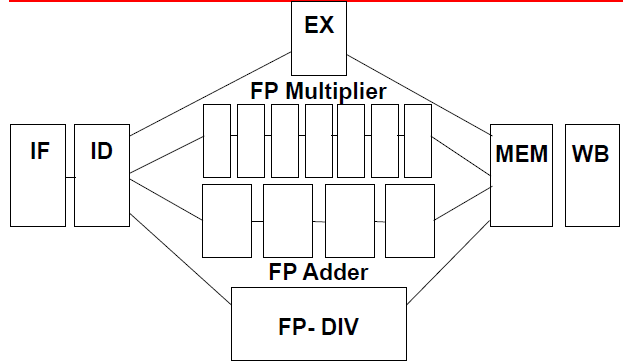
\includegraphics[scale=0.35]{ciclo-instruccion.png}
\end{frame}

\subsection{Ejemplo}
\begin{frame}
\frametitle{Ejemplo}
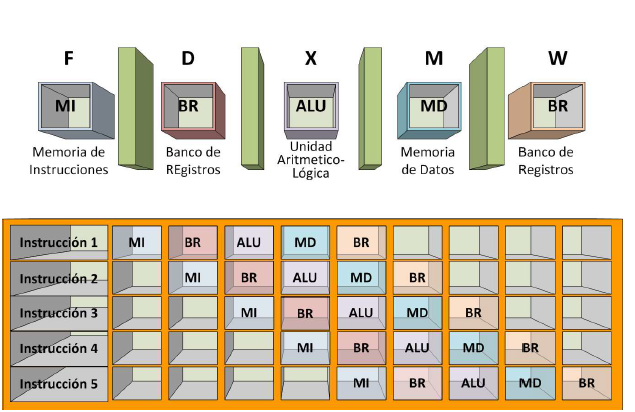
\includegraphics[scale=0.45]{ejemplo-segmentacion.png}
\end{frame}

\section{Assembler}
\subsection{Directivas}
\begin{frame}
\frametitle{Directivas de Ensamblador}
\begin{itemize}
\item Directivas generales
\begin{itemize}
\item \emph{.data}: comienzo de segmento de datos
\item \emph{.text} o \emph{.code}: comienzo de segmento de código
\end{itemize}
\item Las directivas que mas vamos a usar son \emph{.data} y \emph{.code}. Recordar que la memoria de programas y datos son diferentes.
\item Las variables van en el segmento de datos, acordarse antes de empezar a definir variables de escribir la directiva \emph{.data}.
\item Las instrucciones van en el segmento de código. Antes de escribir instrucciones, acordarse de usar la directiva \emph{.code}
\item En un programa puedo intercalar directivas \emph{.data} y \emph{.code}
\item Las etiquetas se definen con un nombre y dos puntos (:), pueden usarse para referenciar partes de un programa (en saltos) como para nombrar variables
\item La CPU empieza a ejecutar instrucción a partir de la posición de memoria 0. Por lo que no es necesario usar la directiva \emph{.org}.
\end{itemize}
\end{frame}

\subsection{Variables}
\begin{frame}
\frametitle{Variables}
Las variables se deben guardar en la memoria de datos.
\begin{itemize}
\item \emph{.word w1}: guarda un word (64-bits, 8 bytes)
\item \emph{.byte b1}: guarda un byte (8-bits, 1 byte)
\item \emph{.word32 n1}: guarda un número(s) de 32 bit (32-bits, 4 bytes)
\item \emph{.word16 n}: guarda un número(s) de 16 bit (16-bits, 2 bytes)
\item \emph{.double f}: guarda un número de punto flotante (64-bits, 8 bytes)
\item \emph{.ascii ``cadena''}: guarda una cadena  ascii
\item \emph{.asciiz ``cadena''}:  guarda una cadena ascii terminada en cero
\end{itemize}
\end{frame}

\subsection{Variables}
\begin{frame}[fragile]
\frametitle{Variables}
\begin{block}{}
\begin{lstlisting}[language=WinMIPS64,basicstyle=\ttfamily,keywordstyle=\color{blue}]
        numero1: .word -50
        numero2: .word 12302
        cadena: .asciiz "Hola Mundo"
\end{lstlisting}
\end{block}
\begin{itemize}
\item Los números pueden ser:
\begin{itemize}
\item Números sin signo, en este caso se guardan en BSS
\item Números con signo, en este caso se guardan en Ca2
\end{itemize}
\item Acordarse, que es nuestro programa el que le da significado a los números
\end{itemize}
\end{frame}

\subsection{Instrucciones}

\begin{frame}
\frametitle{Generalidades}
\begin{itemize}
\item Hay instrucciones especificas para leer y escribir en memoria.
\item Las instrucciones aritmetico-logicas poseen 3 operandos, el primer operando es en el que se va a guardar el resultado, el 2do y 3ro son los parametros de la operación.
\item La instrucción \emph{HALT} se utiliza para detener el simulador.
\item La instrucción \emph{NOP} es una instrucción que no realiza ninguna operación. Mas adelante vamos a ver su utilidad.
\item El registro \emph{r0} siempre vale 0, no se puede cambiar su valor.
\item Las instrucciones de punto flotante solo aceptan como parámetros registros de punto flotante. Salvo las instrucciones de conversión entre punto flotante/punto fijo, no hay instrucciones que acepten diferentes tipos de registros.
\end{itemize}
\end{frame}

\begin{frame}
\frametitle{Instrucciones Generales con valores inmediatos}
Son instrucciones aritmetico/logicas donde el tercer párametro es un valor inmediato.
\begin{itemize}
\item \emph{DADDI r10, r12, 25}: Suma $r12 + 25$ y lo guarda en $r10$
\item \emph{ANDI r8, r10, 11}: Hace la operación AND entre  $r10$ y $11$ y lo guarda en $r8$
\item \emph{ORI r3, r11, 33}: Hace la operación OR entre  $r11$ y $33$ y lo guarda en $r3$
\item \emph{XORI r12, r20, 111}: Hace la operación XOR entre  $r20$ y $111$ y lo guarda en $r12$
\item \emph{SLTI r3, r5, 100}: Si r5 es menor que $100$ entonces $r3$ es $1$, sino $r3$ es $0$
\end{itemize}
Notar que todas las instrucciones finalizan con \emph{I}.
\end{frame}

\begin{frame}
\frametitle{Instrucciones manipulación de Registros}
\begin{itemize}
\item \emph{DADD r1, r2, r3}: Suma $r2 + r3$ y lo guarda en $r1$
\item \emph{DSUB r10, r12, r13}: Resta $r12 - r13$ y lo guarda en $r10$
\item \emph{AND r8, r10, r11}: Hace la operación AND entre  $r10$ y $11$ y lo guarda en $r8$
\item \emph{OR r3, r11, r13}: Hace la operación OR entre  $r11$ y $r13$ y lo guarda en $r3$
\item \emph{XOR r1, r20, r1}: Hace la operación XOR entre  $r20$ y $r1$ y lo guarda en $r1$
\item \emph{SLT r3, r5, r0}: Si $r5$ es menor que $r0$ entonces $r3$ es $1$, sino $r3$ es $0$
\end{itemize}
\end{frame}

\begin{frame}[fragile]
\frametitle{Accesos a memoria}
\begin{itemize}
\item Los accesos a memoria se realizan con 2 instrucciones: LOAD y STORE
\begin{itemize}
\item \emph{LD r10, desplaz(r15)}: Leer desde memoria y guardarlo en el registro $r10$
\item \emph{SD r10, desplaz(r15)}: Guardar en memoria el valor del registro $r10$
\end{itemize}
\item La dirección desde donde leer/escribir se calcula como la suma de $desplaz + r15$
\item $desplaz$ puede ser el nombre de una variable, o un número.
\end{itemize}
\end{frame}

\begin{frame}[fragile]
\frametitle{Accesos a memoria - Variables}
\begin{block}{}
\begin{lstlisting}[language=WinMIPS64,basicstyle=\ttfamily,keywordstyle=\color{blue}]
.data
numero: .word 25
.code
LD r1, numero(r0)
DADDI r5, r0, numero
LD r2, 0(r5)
\end{lstlisting}
\end{block}
\begin{itemize}
\item La instrucción \emph{LD r1, numero(r0)} carga en el registro $r1$, lo que vale la variable numero
\item La instruccion \emph{LD r2, 0(r5)} carga en el registro $r2$, el mismo valor
\begin{itemize}
\item Primero cargamos el registro $r5$ el offset de la variable $numero$
\item La dirección de \emph{LD r2, 0(r5)} es $r5 + 0 = numero + 0 = numero$
\end{itemize}
\end{itemize}
\end{frame}

\begin{frame}[fragile]
\frametitle{Accesos a memoria - Tablas}
\begin{block}{}
\begin{lstlisting}[language=WinMIPS64,basicstyle=\ttfamily,keywordstyle=\color{blue}]
.data
tabla: .word 25, 50, 75, 100
.code
DADD r10, r0, r0   ; r10 = 0
LD r2, tabla(r10)
DADDI r10, r10, 8  ; r10 = r10 + 8
LD r3, tabla(r10)
\end{lstlisting}
\end{block}
\begin{itemize}
\item Podemos obtener los diferentes valores de una tabla
\item El registro $r10$ es nuestro indice en la tabla
\item Debemos incrementar $r10$ en 8, ya que cada elemento de la tabla es de 64bits (8 bytes)
\end{itemize}
\end{frame}

\begin{frame}[fragile]
\frametitle{Accesos a memoria - Tablas II}
\begin{block}{}
\begin{lstlisting}[language=WinMIPS64,basicstyle=\ttfamily,keywordstyle=\color{blue}]
.data
tabla: .word 25, 50, 75, 100
.code
DADDI r11, r0, tabla   ; r11 = tabla
LD r2, 0(r11)
DADDI r11, r11, 8  ; r11 = r11 + 8
LD r3, 0(r11)
\end{lstlisting}
\end{block}

\begin{itemize}
\item Alternativamente podemos realizar lo mismo de antes de otra manera.
\item El registro $r11$ es nuestra posicion en la memoria
\item Debemos incrementar $r11$ en 8, ya que cada elemento de la tabla es de 64bits (8 bytes)
\end{itemize}
\end{frame}



\begin{frame}
\frametitle{Accesos a memoria - Leer Memoria}
Las diferentes variantes de la instrucción \emph{LOAD}:
\begin{itemize}
\item \emph{LD r1, offset(r2)}: Load Doubleword (64 bits)
\item \emph{LB r1, offset(r2)}: Load Byte
\item \emph{LBU r1, offset(r2)}: Load Byte s/signo
\item \emph{LH r1, offset(r2)}: Load Halfword (16 bits)
\item \emph{LHU r1, offset(r2)}: Load Halfword s/signo
\item \emph{LW r1, offset(r2)}: Load Word (32 bits)
\item \emph{LWU r1, offset(r2)}: Load Word s/signo
\end{itemize}
\emph{LB}, \emph{LH} y \emph{LW} extienden el bit de signo.
\end{frame}

\begin{frame}
\frametitle{Accesos a memoria - Escribir Memoria}
Las diferentes variantes de la instrucción \emph{STORE}:
\begin{itemize}
\item \emph{SD r1, offset(r2)}: Store Doubleword
\item \emph{SB r1, offset(r2)}: Store Byte
\item \emph{SH r1, offset(r2)}: Store Halfword
\item \emph{SW r1, offset(r2)}: Store Word
\end{itemize}
\end{frame}

\begin{frame}
\frametitle{Control de Flujo}
\begin{itemize}

\item Salto incondicional:
\begin{itemize}
\item \emph{J etiqueta}:  Saltar a etiqueta
\end{itemize}

\item Salto condicional que compara 2 registros:
\begin{itemize}
\item \emph{BEQ r1, r2, etiqueta}: si r1 = r2 saltar a etiqueta
\item \emph{BNE r1, r2, etiqueta}: si r1 distinto r2 saltar a etiqueta
\end{itemize}

\item Salto condicional que compara con cero:
\begin{itemize}
\item \emph{BEQZ r1, etiqueta}: si r1 = 0 saltar a etiqueta
\item \emph{BNEZ r1, etiqueta}: si r1 no es 0 saltar a etiqueta
\end{itemize}
\end{itemize}
\end{frame}


\section{Ejemplos}
\subsection{Ejemplo 1}

\begin{frame}[fragile]
\frametitle{Ejemplo 1}
\begin{lstlisting}[language=WinMIPS64,basicstyle=\ttfamily,keywordstyle=\color{blue}]
.data
A: .word 1
B: .word 2
.code
   LD   R1, A(R0) ; Cargo R1 con A
   LD   R2, B(R0) ; Cargo R2 con B
   SD   R2, A(R0) ; Guardo en A R2
   SD   R1, B(R0) ; Guardo en A R1
   HALT
\end{lstlisting}

\end{frame}

\subsection{Ejemplo 2}

\begin{frame}[fragile]
\frametitle{Ejemplo 2}
\begin{lstlisting}[language=WinMIPS64,basicstyle=\ttfamily,keywordstyle=\color{blue}]
.data

A: .word 1
B: .word 6

.code
      LD    R1, A(R0)
      LD    R2, B(R0)
LOOP: DSLL  R1, R1, 1
      DADDI R2, R2, -1
      BNEZ  R2, LOOP
      HALT
\end{lstlisting}
\end{frame}

\subsection{Ejemplo 3}
\begin{frame}[fragile]
\frametitle{Manejo de una Tabla}
\tiny{
\begin{lstlisting}[language=WinMIPS64,basicstyle=\ttfamily,keywordstyle=\color{blue}]
.data
        TABLA: .word 20, 1, 14, 3, 2, 58, 18, 7, 12, 11
        NUM:   .word 7
        LONG:  .word 10
.code
        LD     R1, LONG(R0)
        LD     R2, NUM(R0)
        DADD   R3, R0, R0
        DADD   R10, R0, R0
LOOP:   LD     R4, TABLA(R3)
        BEQ    R4, R2, LISTO
        DADDI  R1, R1, -1
        DADDI  R3, R3, 8
        BNEZ   R1, LOOP
        J      FIN
LISTO:  DADDI  R10, R0, 1
FIN:    HALT
\end{lstlisting}
}
\end{frame}
\end{document}

